\section{Parallelization}

\boxlib\ uses a hybrid MPI + OpenMP approach to parallelism.  The
basic idea is that MPI is used to distribute individual boxes across
nodes while OpenMP is used to distribute the work in local boxes to
the cores within a node.  The OpenMP approach in \boxlib\ is optoinally
based on {\em tiling} the box-based data structures.  Both the tiling and
non-tiling approaches to work distribution are discussed below.


\subsection{\boxlib's Non-Tiling Approach In C++}
\label{sec:boxlib0}

At the highest abstraction level, we have {\tt MultiFab} (mulitple
{\tt FArrayBox}es).  A {\tt MultiFab} contains an array of {\tt
  Box}es (a {\tt Box} contains integers specifying the index space it
covers), including {\tt Box}es owned by other processors for the
purpose of communication, an array of MPI ranks specifying which MPI
processor owns each {\tt Box}, and an array of pointers to {\tt
  FArrayBox}es owned by this MPI processor.  The real floating point
data are stored for each {\tt FArrayBox} as one-dimensional arrays,
and can thus be passed across languages, e.g. to Fortran subroutines
for processing. A typical usage of {\tt MultiFab} is as follows,

\begin{lstlisting}
  for (MFIter mfi(mf); mfi.isValid(); ++mfi) // Loop over boxes
  {
    // Get the index space of this iteration
    const Box& box = mfi.validbox(); 

    // Get a reference to the FAB, which contains data and box  
    FArrayBox& fab = mf[mfi];  

    // Get double* of the FAB 
    double* a = fab.dataPtr();

    // Get the index space for the data pointed by the double* 
    // Note "abox" may have ghost cells, and is thus larger than 
    // or equal to "box" obtained using mfi.validbox().
    const Box& abox = fab.box();

    // We can now pass the information to a Fortran routine,
    // which reshapes double* a into a multi-dimensional array 
    // with dimensions specified by the information in "abox".
    // We will also pass "box", which specifies our "work" region.
  }
\end{lstlisting}
A few comments about this code
\begin{itemize}
\item Here the iterator, {\tt mfi}, will perform the loop only over the
   boxes that are local to the MPI task.  If there are 3 boxes on the
   processor, then this loop has 3 iterations.
      
\item {\tt box} as returned from {\tt mfi.validbox()} does not include
   ghost cells.  We can get the indices of the valid zones as {\tt
   box.loVect} and {\tt box.hiVect}.

\item Instead of getting the data pointer explicitly (via {\tt fab.dataPtr()}),
   \castro\ often uses the preprocessor macro {\tt BL\_TO\_FORTRAN(x)} (defined
   in {\tt ArrayLim.H}) to substitute in the data pointer and the {\tt lo}
   and {\tt hi} indices of the multidimensional Fortran array (including ghost cells).
\end{itemize}


\subsection{\boxlib's Current Tiling Approach In C++}
\label{sec:boxlib1}

There are two types of tiling that people discuss.  In {\em logical
tiling}, the data storage in memory is unchanged from how we do things
now in pure MPI.  In a given box, the data region is stored
contiguously).  But when we loop in OpenMP over a box, the tiling
changes how we loop over the data.  The alternative is called {\em
separate tiling}---here the data storage in memory itself is changed
to reflect how the tiling will be performed.  This is not considered
in \boxlib.

We have recently introduced logical tiling into parts of \boxlib.  Examples
that demonstrate the syntax and usage can be found at {\tt
  Tutorials/Tiling\_C}, and {\tt Src/LinearSolvers/C\_CellMG/}.
In our logical tiling approach, a box is logically split into tiles,
and a {\tt MFIter} loops over each tile in each box.  Note that the
non-tiling iteration approach can be considered as a special case of
tiling with the tile size equal to the box size.

\begin{lstlisting}
  bool tiling = true;
  for (MFIter mfi(mf,tiling); mfi.isValid(); ++mfi) // Loop over tiles
  {
    // Get the index space of this iteration
    const Box& box = mfi.tilebox(); 

    // Get a reference to the FAB, which contains data and box  
    FArrayBox& fab = mf[mfi];  

    // Get double* of the FAB 
    double* a = fab.dataPtr();

    // Get the index space for the data pointed by the double*.
    const Box& abox = fab.box();

    // We can now pass the information to a Fortran routine.
  }
\end{lstlisting}
Note that the code is almost identical to the one in \S~\ref{sec:boxlib0}.
Some comments:
\begin{itemize}
\item The iterator now takes an extra argument to turn on tiling
(set to {\tt true}).  There is another interface fo {\tt MFIter}
that can take an {\tt IntVect} that explicitly gives the tile size
in each coordinate direction.

If we don't explictly specify the tile size at the loop, then the
runtime parameter {\tt fabarray.mfiter\_tile\_size} can be used to set it
globally.

\item {\tt .validBox()} has the same meaning as in the non-tile approach,
so we don't use it.  Instead, we use {\tt .tilebox()} to get the
{\tt Box} (and corresponding {\tt lo} and {\tt hi}) for the {\em
current tile}, not the entire data region.

\item When passing into the Fortran routine, we still use the
index space of the entire fab (including ghost cells), as seen in
the {\tt abox} construction.

The Fortran routine will declare a multidimensional array that is of
the same size as the entire box, but only work on the index space
identified by the tile-box ({\tt box}).
\end{itemize}

Let us consider an example.  Suppose there are four boxes---see
Figure~\ref{fig:domain-tiling}.
\begin{figure}[t]
\centering
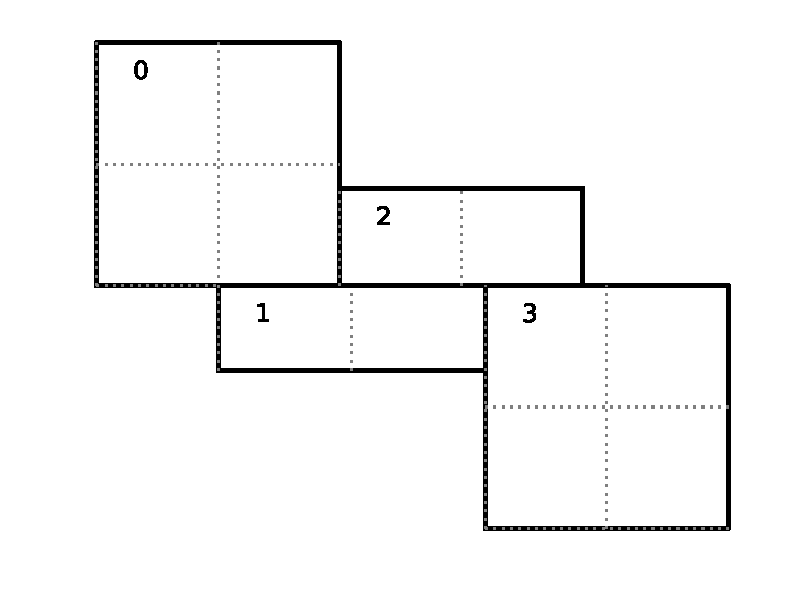
\includegraphics[width=0.8\linewidth]{domain-tile}
\caption{\label{fig:domain-tiling} A simple domain showing 4
  {\tt Box}es labeled 0--3, and their tiling regions (dotted lines)}
\end{figure}
%
The first box is divided into 4 logical tiles, the second and third
are divided into 2 tiles each (because they are small), and the fourth
into 4 tiles.  So there are 12 tiles in total.  The difference between
the tiling and non-tiling version are then:
\begin{itemize}
\item In the tiling version,
the loop body will be run 12 times.  Note that {\tt tilebox} is
different for each tile, whereas {\tt fab} might be referencing the
same object if the tiles belong to the same box.

\item In the non-tiling
version (by constructing {\tt MFIter} without the optional second
argument or setting to {\tt false}), the loop body will be run 4 times
because there are four boxes, and a call to {\tt mfi.tilebox()} will
return the traditional {\tt validbox}.  The non-tiling case is
essentially having one tile per box.
\end{itemize}
 
Tiling provides us the opportunity of a coarse-grained approach for
OpenMP.  Threading can be turned on by inserting the following line
above the {\tt for (MFIter...)} line.
\begin{lstlisting}
  #pragma omp parallel
\end{lstlisting}
Assuming four threads are used in the above example, thread 0 will
work on 3 tiles from the first box, thread 1 on 1 tile from the first
box and 2 tiles from the second box, and so forth.  Note that 
OpenMP can be used even when tiling is turned off.  In that case, the
OpenMP granularity is at the box level (and good performance would need
many boxes per MPI task).

We also note that, independent of whether or not tiling is on, OpenMP
threading can also be started within the function called inside the
{\tt MFIter} loop, rather than at the {\tt MFIter} loop level.  This
was the original way that threading was done in \lmc, but we are in
the process of removing this approach in favor of tiling.

The tile size for the three spatial dimensions can be set by a
parameter, e.g., {\tt fabarray.mfiter\_tile\_size = 1024000 8 8}.  A
huge number like {\tt 1024000} will turn off tiling in that direction.
As noted above, the {\tt MFIter} constructor can also take an explicit
tile size: {\tt MFIter(mfi(mf,IntVect(128,16,32)))}.

Note that tiling can naturally transition from all threads working
on a single box to each thread working on a separate box as the boxes
coarsen (e.g., in multigrid).

The {\tt MFIter} class provides some other useful functions:
\begin{lstlisting}
 mfi.validbox()       : The same meaning as before independent of tiling.
 mfi.growntilebox(int): A grown tile box that includes ghost cells at box
                        boundaries only.  Thus the returned boxes for a
                        Fab are non-overlapping.
 mfi.nodaltilebox(int): Returns non-overlapping edge-type boxes for tiles.
                        The argument is for direction.
 mfi.fabbox()         : Same as mf[mfi].box().
\end{lstlisting}

Finally we note that tiling is not always desired or better.  This
traditional fine-grained approach coupled with dynamic scheduling is
more appropriate for work with unbalanced loads, such as chemistry
burning in cells by an implicit solver.  Tiling can also create extra
work in the ghost cells of tiles.


\subsection{Practical Details in Working with Tiling}

With tiling, the OpenMP is now all in C++, and not in Fortran for all
modules except reactions and initdata.  Note that the OpenMP pragma
does not have a {\tt for}---this is not used when working with an
iterator.

It is the responsibility of the coder to make sure that the routines within
a tiled region are safe to use with OpenMP.  In particular, note that:
\begin{itemize}
\item tile boxes are non-overlapping
\item the union of tile boxes completely cover the valid region of the fab
\item Consider working with a node-centered MultiFab, {\tt ugdnv}, and a
cell=centered MultiFab, {\tt s}:
  \begin{itemize}

  \item with {\tt mfi(s)}, the tiles are based on the cell-centered
  index space.  If you have an $8\times 8$ box, then and 4 tiles, then
  your tiling boxes will range from $0\rightarrow 3$, $4\rightarrow
  7$.

  \item with {\tt mfi{ugdnv}}, the tiles are based on nodal indices,
  so your tiling boxes will range from $0\rightarrow 3$, $4\rightarrow 8$.

  \end{itemize}  
\item When updating routines to work with tiling, we need to understand
the distinction between the index-space of the entire box (which
corresponds to the memory layout) and the index-space of the tile.

  \begin{itemize}

  \item In the C++ end, we pass (usually via the {\tt
  BL\_TO\_FORTRAN()} macro) the {\tt loVect} and {\tt hiVect} of the
  entire box (including ghost cells).  These are then used to allocate
  the array in Fortran as:
  \begin{lstlisting}
    double precision :: a(a_l1:a_h1, a_l2:a_h2, ...)
  \end{lstlisting}
  When tiling is used, we do not want to loop as {\tt do a\_l1, a\_h1},
  but instead we need to loop over the tiling region.  The indices of
  the tiling region need to be passed into the Fortran routine
  separately, and they come from the {\tt mfi.tilebox()} statement.

  \item In Fortran, when initializing an array to 0, do so only over
  the tile region, not for the entire box.  For a Fortran array {\tt a},
  this means we cannot do:
  \begin{lstlisting}
  a = 0.0
  a(:,:,:,:) = 0.0
  \end{lstlisting}
  but instead must do:
  \begin{lstlisting}
  a(lo(1):hi(1),lo(2):hi(2),lo(3):hi(3),:) = 0.0
  \end{lstlisting}
  where {\tt lo()} and {\tt hi()} are the index-space for the tile box
  returned from {\tt mfi.tilebox()} in C++ and passed into the Fortran
  routine.

\item Look at {\tt r\_old\_s} in {\tt Exec/DustCollapse/probdata.f90} as an
  example of how to declare a {\tt threadprivate} variable---this is then used
  in {\tt sponge\_nd.f90}.

\end{itemize}

\end{itemize}


